\chapter{Техническое задание}
\label{cha:analysis}
%
% % В начале раздела  можно напомнить его цель
%
Настоящее техническое задание разработано в рамках учебной программы по курсу <<Технология программирования>> на программное изделие <<Распределенная система обнаружения и фильтрации спама в протоколах POP3, IMAP, SMTP>>. Техническое задание выполняется в соответствии со стандартом ГОСТ 34.602-89 <<Техническое задание на создание автоматизированной системы>>.

\section{Наименование предприятия разработчика и заказчика системы}
Разработчиком системы является Сулимов Александр Сергеевич, студент группы ИУ7-104 кафедры ИУ-7 <<Программное обеспечение вычислительной техники и информационные технологии>> пятого курса очной формы обучения МГТУ им. Баумана.

Заказчиком системы является кафедра ИУ-7 <<Программное обеспечение вычислдительной техники и информационные технологии>> МГТУ им. Баумана (далее Заказчик).

\section{Основания для разработки}
Разработка ведется в рамках выполнения лабораторных работ по курсу <<Технология программирования>> и курсового проекта по курсу <<Распределенные системы обработки информации>> в соответствии с учебным планом МГТУ им. Баумана на 10-й семестр для факультета ИУ кафедры ИУ-7. При выполнении работы учитываются указания, описанные в методических пособиях \cite{metodRomanova}, \cite{metodKKrishenko}.

\section{Сроки выполнения работ по созданию системы}
В соответствии с требованиями Заказчика установлены следующие сроки (указываются номера недель, начиная с 6 февраля 2012 года):

\begin{enumerate}
	\item начало выполнения работ --- 3 неделя (20.02.2012 г.);
	\item конец выполнения работ --- 15 неделя (14.05.2012 г.).
\end{enumerate}

\section{Порядок оформления и предъявления результатов работы по созданию системы}
В \cite{metodKKrishenko} определены следующие требования к оформлению и защите проекта:

\begin{enumerate}
	\item в процессе разработки системы необходимо использовать выделенный Заказчиком репозиторий системы контроля версий;
	\item ответственное лицо со стороны Заказчика ведет контроль выполнения работы по репозиторию, учитывая количество коммитов, определяет процент выполнения проекта;
	\item результаты работ представляются в форме защиты проекта, на которой необходимо предъявить:
		\begin{enumerate}
			\item оформленную, прошитую и подписанную руководителем проекта пояснительную записку;
			\item презентацию в электронном виде в формате PDF;
			\item устаноленное и работающее программное обеспечение с исходными кодами, хранимыми в репозитории;
		\end{enumerate}
	\item при защите программное обеспечение должно быть установленно на компьютерах Заказчика;
	\item для защиты проекта создается комиссия из двух или более ответственных лиц со стороны Заказчика.
\end{enumerate}


\section{Актуальность разрабатываемой системы}
Представленные системы, позволяющие фильтровать почту от нежелательных сообщений, основываются на спам-фильтрах, которые имеют следующие недостатки:

\begin{enumerate}
\item{необходимо обучение;}
\item{история обучения локальная и относится к конкретному пользователю.}
\end{enumerate}

Настоящая разработка должна обеспечить передачу информации между пользователями о признаках обнаруженного спама. Распределенная система обнаружения спама позволит сократить время на обучение спам-фильтров для отдельных пользователей, тем самым повысит удобство использования почтовых клиентов.



\section{Краткое описание предметной области}
За последние десять лет сфера применения спама расширилась, а объем доставки - вырос значительно. Первое время спам рассылался напрямую на единичные адреса пользователей, и его было легко блокировать. Со временем появились высокоскоростные интернет-каналы, которые дали быструю и дешевую возможность массово рассылать спам-сообщения. Модемы пользователей не оснащались средствами защиты от несанкционированного доступа и могли использоваться злоумышленниками из любой точки планеты. Другими словами, модемы ничего не подозревающих пользователей рассылали огромные объемы спама.

Так продолжалось, пока производители аппаратного обеспечения не научились оснащать оборудование средствами защиты от спама, а спам-фильтры не стали более эффективными. Однако спам тоже эволюционировал: усовершенствовались не только способы рассылки, но и приемы, помогающие злоумышленникам обойти спам-фильтры. 

В ходе анализа предметной области были рассмотрены наиболее популярные спам-фильтры и другие механизмы, применяющиеся для фильтрации потока электронной почты от спама.

\subsection{Структура почтовой системы}
Основными элементами почтовой системы являются:
\begin{enumerate}
  \item почтовые клиенты;
  \item почтовые сервера.
\end{enumerate}

В качестве почтовых клиентов могут выступать как отдельные приложения, которые устанавливаются на персональные компьютеры пользователей (например, Microsoft Outlook, Mozilla ThunderBird, The Bat), так и веб-сайты, разработанные поставщиками почтовых услуг. Обычно веб-сайты привязываются к конкретному почтовому серверу, например, mail.ru, gmail.ru, yandex.ru, yahoo.com, hootmail.com.

Стоит отметить, что доступ к перечисленным почтовым серверам может быть настроен и через почтовые клиенты первого типа. На рисунке ~\ref{fig:fig03} представлен типичный интерфейс почтового клиента на примере почтового клиента KMail.

\begin{figure}
  \centering
  \includegraphics[width=\textwidth]{inc/svg/03}
  \caption{Интерфейс почтового клиента KMail на операционной системе Ubuntu}
  \label{fig:fig03}
\end{figure}

Существует множество почтовых серверов и поставщиков почтовых услуг, которые не предоставляют полнофункциональный веб-клиент  для работы  с почтой. В связи с этим большинство предприятий и компаний используют почтовые клиенты для управления почтовыми ящиками, отправкой и получением сообщений.


\section{Существующие аналоги}
В рамках настоящей работы был произведен анализ рынка программных продуктов, позволяющих фильтровать электронную почту от спама. Было выявлено, что существует множество решений позволяющих осуществлять определение нежелательной почты для конкретного пользователя. 

Существует два класса подобных продуктов:
\begin{enumerate}
	\item спам-фильтры на почтовых клиентах;
	\item спам-фильтры на почтовых серверах. 
\end{enumerate}

Спам-фильтры почтовых клиентов основаны на обработке входящих сообщений согласно заданным пользовательским правилам.  Почтовые сервера используют так называемые черные и серые списки доверенных адресов входящей почты.

Таким образом, распределенных систем, позволяющих осуществлять фильтрацию спама обнаружено не было.


\section{Назначение и цели создания системы}
Назначение разработки --- удовлетворить потребности клиентов (пользователей электронной почтой) в получении электронных писем, не относящихся к спаму.

Цели системы:
\begin{enumerate}
	\item информировать пользователя о том, что пришедшее сообщение относится к спаму;
	\item предоставлять пользователю возможность самостоятельно формировать спам-фильтры;
	\item обеспечить доставку писем, не относящихся к спаму.
\end{enumerate}

Таким образом, субъектами разрабытваемой РСОИ являются:

\begin{enumerate}
\item{система <<А>>}, почтовый клиент (MUA);
\item{система <<Б>>}, почтовый сервер (MTA);
\item{система <<C>>}, анти-спам сервер. 
\end{enumerate}

Перечисленные системы в дальнейшем будут также называться субъектами РСОИ или системами-участниками.

На рисунке ~\ref{fig:fig01} представлена структура предметной области и ее составные части.

\begin{figure}
  \centering
  \includegraphics[width=\textwidth]{inc/dia/rsoi-structure}
  \caption{Структура предметной области}
  \label{fig:fig01}
\end{figure}


\subsection{Система <<А>>}
Целью систем данного типа является предоставление удобного пользовательского интерфейса для работы с электронной почтой. С точки зрения почтовой системы представляют собой MUA --- программное обеспечение, устанавливаемое на компьютере пользователя и предназначенное для получения, написания, отправки и хранения сообщений электронной почты одного или нескольких пользователей (в случае, например, нескольких учётных записей на одном компьютере) или нескольких учётных записей одного пользователя. 

Системы <<А>> бывают двух типов в зависимости от протокола получения входящих сообщений:
\begin{enumerate}
\item{POP3;}
\item{IMAP.}
\end{enumerate}

Протокол POP3 подразумевает передачу входящих сообщений почтовым сервером и сохранение электронных писем на локальном компьютере пользователя. При использовании POP3 клиент подключается к серверу только на промежуток времени, необходимый для загрузки новых сообщений. При использовании IMAP соединение не разрывается, пока пользовательский интерфейс активен, а сообщения загружаются только по требованию клиента. Это позволяет уменьшить время отклика для пользователей, в чьих ящиках имеется много сообщений большого объёма.
Протокол POP требует, чтоб текущий клиент был единственным подключенным к ящику. IMAP позволяет одновременный доступ нескольких клиентов к ящику и предоставляет клиенту возможность отслеживать изменения, вносимые другими клиентами, подключенными одновременно с ним.


\subsection{Система <<Б>>}
Системы аккумулируют информацию необходимую для фильтрации электронной почты пользователя от спама. Целевые пользователи систем <<А>> должны зарегистрироваться в одной из систем типа <<Б>>. Такие системы получают информацию от пользователей относительно того, являются ли те или иные сообщения спамом или нет. В зависимости от полученных данных от пользователей в системах типа <<Б>> аккумулируется база данных, содержащая список адресов, с которых рассылаются спам-сообщения.

При получении почты системой <<А>> посылается запрос связанной с ней системой <<Б>>, которая должна классифицировать входящее сообщение на наличе спама.

Системы типа <<Б>> взаимодействуют между собой, таким образом пользователи, входящие в состав РСОИ, обладают суммарной информацией о всех спам-рассылках в рамках текущей сети. Так как с каждым пользователем системы <<А>>  в определенный момент времени связан лишь один антиспам сервер, то существует возможность составлять персональные спам-списки для каждого пользователя. 


\subsection{Система <<В>>}
 Системы данного типа отвечает за отправку почты и представляют собой почтовые сервера, которые обычно выполняют роль MTA и MDA. Некоторые почтовые сервера (программы) выполняют роль как MTA, так и MDA, некоторые подразумевают разделение на два независимых сервера: сервер-MTA и сервер-MDA (при этом, если для доступа к почтовому ящику используются различные протоколы — например, POP3 и IMAP, — то MDA в свою очередь может быть реализован либо как единое приложение, либо как набор приложений, каждое из которых отвечает за отдельный протокол).

 \section{Требования к системе}
 \subsection{Требование к системе вцелом}

 Разрабатываемое ПО должно удовлетворять следующим требованиям:

 \begin{enumerate}
 	\item все системы в РСОИ могут быть в одном или нескольких экземплярах, включение новой системы в РСОИ не должно приводить к нарушению работы других субъектов;
 	\item программное обеспечение для систем каждого типа должно 	поддерживать функционирование системы в режиме:
 		\begin{enumerate}
 			\item системы <<А>> --- периодическая работа в зависимости от желаний пользователя, в том числе поддерживать режим 24/7/365;
 			\item системы <<Б>> --- режим 24/7/365;
 			\item системы <<В>> --- режим 24/7/365.
 		\end{enumerate}
 	\item системы должны быть устойчивы к отключениям питания и другим техническим сбоям, которые могут привести к нарушению нормального фуннкционирования систем;
 	\item выход из строя одного субъекта РСОИ не должен приводить к сбою в работе других систем;
 	\item для корректного взаимодействия систем в РСОИ должен быть разработан протокол, однозначно определяющий содержание всех запросов и возможные сценарии совместной работы систем с указанием возможных состояний каждой из систем и состояний заявок в них.
 \end{enumerate}

 \subsection{Требования к функциональным характеристикам}
 К разрабатываему ПО выдвигаются следующие функциональные требования:
 \begin{enumerate}
 	\item время отклика на запрос пользователя не должно превышать 3 секунд;
 	\item время ожидания запросов для различных систем должно настраиваться с помощью конфигурационных файлов отдельно;
 	\item системы типа <<Б>> должны функционировать и поддерживать указанное время отклика для 50 одновременно подключенных клиентов-систем типа <<А>>;
 	\item указанные требования к временным задержкам должны соблюдаться для систем всех типов при одноверменной работе с 5-10 системами партнерами.
 \end{enumerate}

 \subsection{Требования по реализации}
 При разработке РСОИ участвующие системы реализуются в виде независимых программных продуктов, использующих общий протокол прикладного уровня для взаимодействия друг с другом. 

 К каждому из программных продуктов предъявляются следующие тербования:
 \begin{enumerate}
 	\item разрабатываемое ПО должно предоставлять удобный пользовательский интерфейс для работы администраторов и пользователей;
 	\item интерфейс систем должен быть реализован как WEB-интерфейс;
 	\item каждая заявка должна обладать уникальным идентификатором в рамках одного субъекта РСОИ;
 	\item в качестве транспортного протокола системы должны использовать почтовые протоколы SMTP для отправки POP3/IMAP для получения сообщений и протоколы удаленного вызова процедур XML-RPC;
 	\item в качестве языка разметки могут быть использованы языки XML, либо JSON;
 	\item для хранения данных о пользователях, сообщениях, спаме необходимо использовать СУБД Postgres. Непосредственный доступ к базе данных одной системы должен быть закрыт для систем партнеров и клиентов.
 \end{enumerate}


\section{Функциональные требования к системе}
\subsection{Функциональные требования к системам типа <<А>>}
Система <<А>> должна предоставлять следующие функции:
\begin{enumerate}
	\item аутентификация и авторизация пользователей;
	\item просмотр входящих сообщений пользователями;
	\item регистрация анти-спам сервера через панель настроек;
	\item оповещение связанного анти-спам сервера о наличии спам сообщений;
	\item просмотр сообщений, которые являются спамом по данным РСОИ;
	\item добавление адресатов в доверенный список, после чего сообщения от данных пользователей не классифицируются как спам;
	\item изменение способа получения входящих сообщений (протокол IMAP, POP3).
\end{enumerate}



\subsection{Функциональные требования к системам типа <<Б>>}
Система <<Б>> должна предоставлять следующие функции:
\begin{enumerate}
	\item аутентификация и авторизация пользователей;
	\item настройка спам-фильтров на стороне почтового сервера;
	\item настройка серых списков;
	\item настройка черных списков.
\end{enumerate}


\subsection{Функциональные требования к системам типа <<В>>}
Система <<В>> должна предоставить следующие функции:
\begin{enumerate}
	\item аутентификация и авторизация пользователей;
	\item просмотр списка подключенных почтовыхъ клиентов к данному анти-спам серверу;
	\item просмотр списка адресатов, признанных за спамеров;
	\item настройка списка адресатов;
	\item просмотр статуса вхощего сообщения;
	\item отмена обработки сообщения: доставка клиенту, удаление.
\end{enumerate}



\section{Входные параметры}
\subsection{Входные параметры систем типа <<А>>}
Система должна содержать следующую информацию о анти-спам сервере (система типа <<В>>):
\begin{enumerate}
	\item идентификатор системы;
	\item название системы;
	\item веб-адрес системы;
	\item адрес электронной почты системы;
	\item адрес XML-RPC сервера системы.
\end{enumerate}

Система должна содержать следующую информацию о почтовом сервере (система типа <<Б>>):
\begin{enumerate}
	\item идентификатор;
	\item название системы;
	\item веб-адрес системы;
	\item адрес электронной почты системы;
	\item адрес исходящей почты;
	\item адрес входящей почты и протокол ее получения.
\end{enumerate}

Система должна содержать следующую информацию о прокси-серверах POP3 и IMAP:
\begin{enumerate}
	\item веб-адрес сервера.
\end{enumerate}

Система должна содержать следующую информацию о пользователе:
\begin{enumerate}
	\item логин(уникальный идентификатор, адрес электронной почты);
	\item пароль;
	\item время последнего входа в систему;
	\item способ работы в настоящий момент времени (автономно, либо удаленно).
\end{enumerate}

Система должна содержать следующую информацию о входящем сообщении:
\begin{enumerate}
	\item уникальный идентификатор сообщения в рамках системы;
	\item наименование отправителя/получателя;
	\item контент сообщения (тема и тело сообщения);
	\item маркер спама, установленный пользователем (оценка от 0\% до 100\%);
	\item время получения сообщения.
\end{enumerate}

Система должна содержать следующую информацию об ошибках в работе:
\begin{enumerate}
	\item уникальный идентификатор ошибки в рамках системы;
	\item время возникновения;
	\item код ошибки;
	\item логин пользователя;
	\item адрес почтового сервера, адрес анти-спам сервера, адреса прокси серверов.
\end{enumerate}

\subsection{Входные параметры систем типа <<Б>>}

Система должна содержать следующую информацию о сообщении:
\begin{enumerate}
	\item уникальный идентификатор сообщения в рамках системы;
	\item адрес отправителя;
	\item адрес получателя;
	\item контент сообщения (текст и тело).
\end{enumerate}

Система должна знать следующую информацию об администраторах системы:
\begin{enumerate}
	\item логин;
	\item пароль.
\end{enumerate}

Система должна содержать следующую информацию об ошибках в работе:
\begin{enumerate}
	\item уникальный идентификатор ошибки в рамках системы;
	\item время возникновения;
	\item код ошибки.
\end{enumerate}

\subsection{Входные параметры систем типа <<В>>}
Система должна знать следующую информацию о сообщении:
\begin{enumerate}
	\item уникальный идентификатор сообщения в рамках системы;
	\item адрес отправителя;
	\item адрес получателя;
	\item степень доверия получателя отправителю (10\%...60\%).
\end{enumerate}

Система должна знать следующую информацию о других анти-спам серверах:
\begin{enumerate}
	\item адреса анти-спам серверов системы.
\end{enumerate}

Система должна содержать следующую информацию об ошибках в работе:
\begin{enumerate}
	\item уникальный идентификатор ошибки в рамках системы;
	\item время возникновения;
	\item код ошибки;
	\item статус сообщений.
\end{enumerate}

\section{Выходные параметры}
Выходными параметрами для систем являются:

\begin{enumerate}
	\item визуальное отображение информации о пользователе;
	\item визуальное отображение результатов классификации сообщений;
	\item визуальное отображение списков взаимодействующих систем.
\end{enumerate}

\section{Требования к составу и параметрам технических средств}
Минимальные требования к программно-аппаратному обеспечению для рабочей станции системы типа <<А>>:

\begin{enumerate}
	\item тактовая частота  --- не менее $3,0 \text{ГГц}$;
	\item оперативная память --- не менее $1 \text{Гб}$;
	\item требования к операционной системе:
	\begin{enumerate}
		\item Windows XP и старше;
		\item Mac OS X 10.5 и старше;
	\end{enumerate}
	\item свободное пространство на жестком диске не менее 10 Гб для операционной системы;
	\item свободное пространство на жестком диске не менее 200 Мб для программного обеспечения;
	\item Ethernet-адаптер стандарта 1000BASE-T для доступа к сети;
	\item веб-браузер;
	\item интерпретатор языка Python (для работы прокси).
\end{enumerate}

Минимальные требования к программно-аппаратному обеспечению для почтовых серверов систем типа <<Б>>:

\begin{enumerate}
	\item тактовая частота  --- не менее $2\times3,0$ ГГц; 
	\item оперативная память --- не менее $4$ Гб;
	\item требования к операционной системе:
	\begin{enumerate}
		\item Windows Server 2003 и старше;
		\item дистрибутив линукс с ядром версии 2.6:3.0;
	\end{enumerate}
	\item свободное пространство на жестком диске не менее 10 Гб для операционной системы;
	\item свободное пространство на жестком диске не менее 200 Мб для программного обеспечения;
	\item Ethernet-адаптер стандарта 1000BASE-T для доступа к сети;
	\item интерпретатор языка Python (для работы почтового сервиса);
	\item СУБД Postgres;	
	\item платформа Django для веб-интерфейса.
\end{enumerate}

Минимальные требования к программно-аппаратному обеспечению для анти-спам серверов систем типа <<В>>:

\begin{enumerate}
	\item тактовая частота  --- не менее $2\times3,0 \text{ГГц}$; 
	\item оперативная память --- не менее $4 \text{Гб}$;
	\item требования к операционной системе:
	\begin{enumerate}
		\item Windows Server 2003 и старше;
		\item дистрибутив линукс с ядром версии 2.6:3.0;
	\end{enumerate}
	\item свободное пространство на жестком диске не менее 10 Гб для операционной системы;
	\item свободное пространство на жестком диске не менее 200 Мб для программного обеспечения;
	\item Ethernet-адаптер стандарта 1000BASE-T для доступа к сети;
	\item интерпретатор языка Python (для работы прокси);
	\item платформа Django для веб-интерфейса;
	\item СУБД Postgres.
\end{enumerate}

\section{Сценарии функционирования системы}
\subsection{Общий сценарий функционирования РСОИ}
Общий сценарий функционирования системы сожно представить следующим образом:

\begin{enumerate}
  \item Пользователь проходит процедуру авторизации в системе (вводит логин и пароль в почтовом клиенте), так как регистрация осуществляется непосредственно при создании аккаунта электронной почты на некотором почтовом сервере.
  \item Пользователь иницирует запрос для получения входящей почты от других пользователей (не обязательно подключенных к данной РСОИ).
  \item Система почтового сервера, получив запрос сообщений из почтового ящика, проверяет идентификационную информацию о пользователе.
  \item После проверки начинается отправка входящих сообщений по протоколам IMAP или POP3 в зависимости от настроек почтового клиента.
  \item Почтовый клиент посылает входящую почту связанному с ним анти-спам серверу, не отображая принятые сообщения конечному пользователю.
  \item Анти-спам сервер для каждого адреса сообщений входящей почты производит опрос других анти-спам серверов, входящих в состав РСОИ. На основании полученных ответов выдается результат о том, является ли конкретное сообщение спамом или нет.
  \item Анти-спам сервер возвращает результат почтовому клиенту;
  \item Почтовый клиент, получив результат анализа на присутствие спама корректным образом отображает входящую почту: сообщения принятые за спам перемещаются в необходимую директорию.
\end{enumerate}

\subsection{Сценарии функционирования систем <<Почтовый клиент>> (системы типа <<А>>)}

\subsubsection{Вход в систему}

Действие должно выполняться пользователем и должно состоять из следующих шагов:
\begin{enumerate}
  \item Пользователь переходит во вкладку <<Вход>> и заполняет поля <<Имя пользователя>>, <<Email>> и <<Пароль>>.
  \item Пользователь указывает настройки почтового сервера:
    \begin{itemize}
      \item тип учетной записи (POP3, IMAP);
      \item сервер входящей почты;
      \item сервер исходящей почты;
      \item номера портов сервера IMAP (по умолчанию 143), SMTP (по умолчанию 25);
      \item тип шифрованного подключения (SSL, TLS, нет);
      \item длительность ожидания ответа от сервера.
    \end{itemize}
  \item Пользователь указывает настройки анти-спам сервера: адрес.
  \item Производится соединение с почтовым серевером для проверки введенных пользователем данных.
  \item Альтернативный сценарий: в случае если сочетание <<email - пароль>> пользователя введено неверно, система выводит информацию об ошибке в интерфейсе пользователя.
\end{enumerate}

\subsection{Выход из системы}
Действие должно выполняться пользователем и должно состоять из следующих шагов:
\begin{enumerate}
  \item Пользователь нажимает на кнопку <<Выход>>.
  \item Все запущенные процессы останавливаются: производится разрыв соединения с анти-спам сервером, почтовым сервером.
  \item Альтернативный сценарий: аналогичные действия производятся при закрытии окна интерфейса пользователем.
\end{enumerate}

\subsubsection{Получение почты}
Действие должно выполняться авторизованным пользователем и должно состоять из следующих шагов:

\begin{enumerate}
  \item Пользователь нажимает на кнопку <<Получение почты>>.
  \item Почтовый клиент отображает новые полученные входящие сообщения.
  \item Альтернативный сценарий: в случае отсутствия новых входящих сообщений система выводит соответствующую информацию в интерфейсе пользователя.
\end{enumerate}

\subsubsection{Классификация сообщения как спам}
Действие должно выполняться авторизованным пользователем и должно состоять из следующих шагов:

\begin{enumerate}
  \item Пользователь выделяет определенное входящее сообщение из списка и нажимает на кнопку <<Классифицировать сообщение как спам>>.
  \item Система посылает анти-спам серверу информацию о том, что сообщение конкретного адресата было классифицировано текущим пользователем как спам.
  \item Альтернативный сценарий: в случае потери связи с анти-спам сервером система выводит информацию о невозможности в текущий момент связаться с анти-спам сервером, информация будет отправлена позднее.
\end{enumerate}

\subsubsection{Классификация сообщения как не спам}
Действие должно выполняться авторизованным пользователем и должно состоять из следующих шагов:

\begin{enumerate}
  \item Пользователь выделяет определенное входящее сообщение из списка и нажимает на кнопку <<Классифицировать сообщение как НЕ спам>>.
  \item Система посылает анти-спам серверу информацию о том, что сообщение конкретного адресата было классифицировано текущим пользователем как спам.
  \item Альтернативный сценарий: в случае потери связи с анти-спам сервером система выводит информацию о невозможности в текущий момент связаться с анти-спам сервером, информация будет отправлена позднее.
\end{enumerate}


\subsubsection{Автоматическая классификация сообщений}
Действие должно выполняться системой на основе локальных фильтров созданных пользователем, и должно состоять из следующих шагов:

\begin{enumerate}
  \item При поступлении входящей почты происходит автоматический анализ почты в соответствии с заданными пользовательчкими фильтрами.
  \item В результате анализа все входящие сообщения классифицируются на спам и не спам.
  \item Сообщения, принятые за спам, помещаются в специальную директорию.
  \item Система отлавливает событие перемещения сообщений в папку спама и посылает связанному анти-спам серверу информацию об обнаруженных спам-сообщениях.
  \item Альтернативный сценарий: в случае потери связи с анти-спам сервером система выводит информацию о невозможности в текущий момент связаться с анти-спам сервером. Отображается пустой список, либо список из локального кэша.
\end{enumerate}

\subsubsection{Просмотр списка спам-адресатов}
Действие должно выполняться авторизованным пользователем и должно состоять из следующих шагов:

\begin{enumerate}
  \item Пользователь нажимает на кнопку <<Просмотр спам-адресатов>>.
  \item Система посылает анти-спам серверу запрос о получении списка адресов, с которых предположительно рассылаются спам-сообщения.
  \item После получения ответа от анти-спам сервера происходит отображение таблицы содержащей информацию о списке адресатов-спамеров с указанием степени  доверия для текущего пользователя.
  \item Альтернативный сценарий: в случае потери связи с анти-спам сервером система выводит информацию о невозможности в текущий момент связаться с анти-спам сервером. Отображается пустой список, либо список из локального кэша.
\end{enumerate}


\subsubsection{Журналирование действий}
Действие должно выполняться в автоматическом режиме системой и основывается на ведение журналов, в которых хранится информация о том в какое время пользователь совершил определенные действия.

\subsection{Сценарии функционирования систем <<Почтовый сервер>> (системы типа <<Б>>)}
Все сценарии выполняются пользователем с ролью <<Администратор>>.

\subsubsection{Вход в систему}

Действие должно выполняться пользователем и должно состоять из следующих шагов:
\begin{enumerate}
  \item Пользователь переходит во вкладку <<Вход>> и заполняет поля <<Имя пользователя>> и <<Пароль>>.
  \item Производится запись в системном журнале о времени авторизации.
  \item Альтернативный сценарий: в случае если сочетание <<имя пользователя - пароль>> пользователя введено неверно, система выводит информацию об ошибке в интерфейсе пользователя.
\end{enumerate}

\subsection{Выход из системы}
Действие должно выполняться пользователем и должно состоять из следующих шагов:
\begin{enumerate}
  \item Пользователь нажимает на кнопку <<Выход>>.
  \item Производится пересылка на страницу авторизации.
  \item Альтернативный сценарий: аналогичные действия производятся при закрытии окна интерфейса пользователем.
\end{enumerate}

\subsubsection{Настройка параметров фильтрации спама}
В зависимости от настроек могут быть заданы либо черные, либо серые списки недоверенных адресатов. Почта от отправителей из этих списков будет классифицироваться как спам.

Действие должно выполняться авторизованным пользователем и должно состоять из следующих шагов:
\begin{enumerate}
  \item Пользователь заходит на вкладку <<Настройка спам-списков>>.
  \item Пользователь выбирает тип списка (черный, серый) и добавляет адреса потенциально опасных пользователей почтовой системы.
\end{enumerate}

\subsection{Сценарии функционирования систем <<Анти-спам сервер>> (системы типа <<В>>)}
Все сценарии выполняются пользователем с ролью <<Администратор>>.

Действие должно выполняться пользователем и должно состоять из следующих шагов:
\begin{enumerate}
  \item Пользователь переходит во вкладку <<Вход>> и заполняет поля <<Имя пользователя>> и <<Пароль>>.
  \item Производится запись в системном журнале о времени авторизации.
  \item Альтернативный сценарий: в случае если сочетание <<имя пользователя - пароль>> пользователя введено неверно, система выводит информацию об ошибке в интерфейсе пользователя.
\end{enumerate}

\subsubsection{Выход из системы}
Действие должно выполняться пользователем и должно состоять из следующих шагов:
\begin{enumerate}
  \item Пользователь нажимает на кнопку <<Выход>>.
  \item Производится пересылка на страницу авторизации.
  \item Альтернативный сценарий: аналогичные действия производятся при закрытии окна интерфейса пользователем.
\end{enumerate}

\subsubsection{Настройка списка анти-спам серверов для взаимодействия}
Действие должно выполняться авторизованным пользователем и должно состоять из следующих шагов:
\begin{enumerate}
  \item Пользователь переходит на вкладку <<Настройка>>.
  \item На странице настройки пользователь вводит информацию об имеющихся в РСОИ других анти-спам серверах, указывая их адреса.
  \item При добавлении нового анти-спам сервера происходит тестовое соединение систем друг с другом.
  \item Для успешной работы должен прийти ответ от добавляемого сервера за определенный промежуток времени.
  \item Альтернативный сценарий: если добавляемый сервер не ответил в определенный промежуток времени, то система выводит информацию в интерфейсе пользователя.
\end{enumerate}

\subsubsection{Редактирование списка спам-адресатов}
Действие должно выполняться авторизованным пользователем и должно состоять из следующих шагов:
\begin{enumerate}
  \item Пользователь переходит на вкладку <<Спам-адресаты>>.
  \item На данной странице отображается таблица, в которой содержится информация о списках спамеров каждого пользователя данным анти-спам сервером.
  \item Альтернативный сценарий: если не удалось по каким-либо причинам получить информацию из базы данных, то система выводит сообщение об ошибке в интерфейсе пользователя.
\end{enumerate}

\subsubsection{Просмотр списка почтовых клиентов}
Действие должно выполняться авторизованным пользователем и должно состоять из следующих шагов:
\begin{enumerate}
  \item Пользователь переходит на вкладку <<Клиенты>>.
  \item На данной странице отображается таблица, в которой содержится информация о клиентах, связанных с данной системой.
\end{enumerate}

\subsubsection{Блокирование почтового клиента}
Существует возможность блокировать определенные почтовые клиенты и не учитывать информацию от них при классификации входящей почты. Для того действие должно выполняться авторизованным пользователем и должно состоять из следующих шагов:

\begin{enumerate}
  \item Пользователь переходит на вкладку <<Клиенты>>.
  \item На данной странице отображается таблица, в которой содержится информация о клиентах, связанных с данной системой.
  \item Пользователь выбирает клиента из списка и нажимает на кнопку <<Блокировать>>.
\end{enumerate}

\section{Состав и содержание работ по созданию системы}
В таблице \ref{tab:sostav} представлен состав работ по созданию РСОИ <<Распределенная система обнаружения и фильтрации спама в протоколах POP3, IMAP, SMTP>>. Перечень работ соответствует требованиям Заказчика.

\begin{table}[ht]
  \caption{Перечень работ по созданию РСОИ}
  \begin{tabular}{|p{0.70\textwidth}|c|}
  \hline
  Выполняемая работа & Срок выполнения\\
  \hline
  Исследование объектов автоматизации, сбор сведений о существующих аналогах & 1 неделя \\
  \hline
  Разработка технического задания & 4 неделя \\
  \hline
  Разработка пилотного проекта по выбранному варианту РСОИ & 6 неделя \\
  \hline
  Разработка окончательных решений по выбранным структурам, разработка конечных вариантов процедур и заглуушек систем-партнеров & 8 неделя \\
  \hline
  Разработка пользовательского интерфейса & 12 неделя \\ 
  \hline
   Создание документации & 12 неделя \\
  \hline
  Отладка проекта, подготовка к защите & 14 неделя \\
  \hline
  Защита проекта & 15 неделя\\
  \hline
  \end{tabular}
  \label{tab:sostav}
\end{table}


\section{Порядок контроля и приемки системы}
При разработке системы необходимо произвести следующие испытания:
\begin{enumerate}
	\item тестирование логики работы систем всех типов <<А>>, <<Б>>, <<В>>: при тестировании системы одного типа системы другого типа представляются в виде заглушек, работающих по строго заданным сценариям;
	\item тестирование нормальной совместной работы систем <<А>>, <<Б>>, <<В>>: проверяются различные сценарии работы при корректных входных данных, предполагаемые результаты работы сравниваются с реально полученными;
	\item испытание РСОИ на отказоустойчивость: имитирование таких событий как отключение питания, выход из строя других систем в составе РСОИ, поступление запросов с ошибочной или противоречивой информацией, поступление запросов в неверном формате и порядке.
\end{enumerate}


\section{Требования к документации}
Разработка, установка и внедрение системы должны сопровождаться следующими документами:

\begin{enumerate}
	\item руководство по установке, настройке систем всех типов при развертывании РСОИ;
	\item руководство по использованию систем <<А>> для пользователей;
	\item руководство по использованию систем <<Б>>, <<В>> для администраторов.
\end{enumerate}



%%% Local Variables:
%%% mode: latex
%%% TeX-master: "rpz"
%%% End:
